\documentclass[tikz]{standalone}
\usepackage{tikz}
\usetikzlibrary{shapes}

\begin{document}

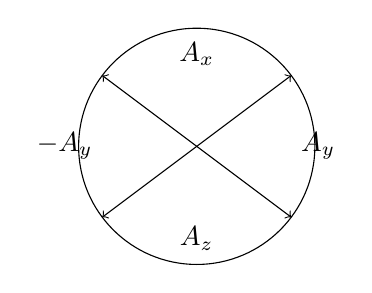
\begin{tikzpicture}[scale=1.5]

% 画圆
\draw (0,0) circle (1);

% 画箭头
\draw[->] (0,0) -- (0.8,0.6);
\draw[->] (0,0) -- (-0.8,0.6);
\draw[->] (0,0) -- (0.8,-0.6);
\draw[->] (0,0) -- (-0.8,-0.6);

% 标记文字
\node[above] at (0,0.6) {$A_x$};
\node[below] at (0,-0.6) {$A_z$};
\node[right] at (0.8,0) {$A_y$};
\node[left] at (-0.8,0) {$-A_y$};

\end{tikzpicture}

\end{document}
